%%
%% Dit is het hoofddocument: compileer dit met latex of xelatex en je krijgt de gehele pdf
%%
\documentclass[a4paper,11pt]{article}

\usepackage{subfig}
\usepackage{wrapfig}% product wrapfigure and wraptable
\usepackage[dutch]{babel}
\usepackage{graphicx}
\usepackage[colorlinks]{hyperref}
\usepackage[prependcaption,colorinlistoftodos,obeyFinal]{todonotes}% when generating final (documentclass option) skip notes
\usepackage{pgfgantt}
\usepackage{pdflscape}
\usepackage[a4paper]{geometry}

\bibliographystyle{alpha}

\usepackage{hyperref}

\author{Guus Bonnema, Stefan Versluys, Jeroen Kleijn}
\date{24/09/14}

\title{Plan van aanpak voor \xmas\ ontwerp tool}


%% Document is in subdocumenten gesplitst.

\begin{document}

\selectlanguage{dutch}

\newcommand{\xmas}{x\textsc{mas}}%

\maketitle

\listoftodos

\begin{abstract}
 Dit document is het plan van aanpak voor het ABI (afstudeer project bachelor
 informatica). De opdrachtgever is Bernard van Gastel en de begeleider is
 Freek Verbeek. Het project is gericht op het verbeteren van een bestaand
 chip ontwerp tool op de aspecten platform onafhankelijkheid, uitbreidbaarheid,
 en integratie met de analyse tools.

 Het plan is gebouwd op basis van een hybride agile aanpak , een aanpak dat
 moet passen bij de noden van het team alsook voor het probleem.

 De domeinanalyses omvatten onderzoek van deelgebieden uit de productcontext
 dat alternatieven voor oplossingen aan het licht moeten brengen. Op die manier
 kunnen keuzes wetenschappelijk onderbouwd worden en kan er aan de opdrachtgever
 verantwoord advies geven worden.

\end{abstract}

%%
%% Dit is een subdocument van het projectplan.
%%

\section{Opdracht}

\subsection{Business case}

De projectaanvraag voor dit project van Bernard van Gastel en
Freek Verbeek verwoordt de business case in de projectaanvraag
als volgt.

\begin{quote}
    \small\sf
    ``De Network-on-Chip (NoC) groep van de OU doet onderzoek
    naar nieuwe methoden om NoC ontwerpen (moderne manier van
    ontwerpen van processoren) foutvrij te krijgen met behoud van
    efficiëntie. De NoC groep heeft een aantal tools ter ondersteuning
    van het onderzoek gemaakt (met ondersteuning van vele studenten
    projecten), voornamelijk WickedXmas. Deze tool stelt de
    gebruiker in staat om chip ontwerp te maken/bewerken/genereren
    in de visuele xMAS taal van Intel, en vervolgens een aantal door
    ons ontwikkelde tools op los te laten (bv symbolische analyse,
    deadlock checker, etc).
    De huidige tool heeft een aantal problemen:

    \begin{itemize}
	\item niet modulair opgezet (waardoor uitbreidingen moeizaam gaan)
	\item op Windows API gebaseerd (waardoor de onderzoekers die
	    gebruik maken van Mac het lastig kunnen gebruiken)
	\item moeizame integratie met tools: WickedXmas is nu geschreven
	    in C\#, en lijkt moeilijk te integreren met onze C/C++ tools
	\item geen documentatie
    \end{itemize}

    Deze problemen moeten opgelost worden, danwel door een grote
    refactoring van de bestaande code, danwel door het opnieuw
    bouwen.''
\end{quote}

Omdat dit het afstudeerproject is van drie studenten, zijn er geen financi\"ele overwegingen.
De kosten die er zijn (inzet opdrachtgever en begeleider) vallen onder het afstuderen. Deze kosten
zijn al gedekt als onderdeel van de cursus Afstudeerproject Bachelor Informatica (ABI).

De baten zijn vooral betere onderhoudbaarheid en uitbreidbaarheid en een bredere ondersteuning van platformen.
Deze verbeteringen ondersteunen met name het chipontwerponderzoek aan universiteiten en bedrijven. Dankzij een betere integratie
tussen ontwerptool en verificatietools optimaliseren de onderzoekers hun workflow. Het aantal handelingen
dat zij moeten uitvoeren is minder dan met het huidig tool en de directe feedback in de user interface
versnelt het lokaliseren en verhelpen van fouten in een ontwerp.

\subsection{Vision}\label{sec: vision}

Deze sectie geeft aan wat de opdrachtgever ziet als ideale uitkomst van het project. Het ontwerptool is
bedoeld voor wetenschappers van universiteiten en van bedrijven (o.a. Intel). Onderzoekers op verschillende
platformen kunnen het ontwerptool gemakkelijk downloaden, installeren en gebruiken. Het tool toont op verzoek
tijdens het ontwerp fouten die door de verificatietools zijn gevonden.

Het programma is goed gestructureerd, uit te breiden met nieuwe verificatietools en NoC onderzoekers
kunnen gemakkelijk nieuwe primitieven defini\"eren. Ten slotte kunnen de \xmas\ -onderzoekers onze bestanden
converteren naar een ander formaat zoals Verilog.

\subsection{Stakeholders}

Opdrachtgever is Bernard van Gastel van de Open Universiteit. Begeleider is Freek Verbeek van de Open Universiteit.
De doelgroep voor gebruikers van het ontwerptool bestaat uit medewerkers van universiteiten en onderzoekers van bedrijven zoals
Intel en LLC. Een kleine groep van \xmas\ -onderzoekers van zowel de universiteit als bedrijven gebruiken het ontwerptool
vanuit de optiek van onderzoek naar verbetering van NoC ontwerp. Doelstellingen voor deze groep zijn chip import
en export van bestandsformaten (zoals Verilog) en verificatie van aspecten van correctheid (deadlock, livelock,
syntactische of semantische checks). Bernard en Freek nemen het onderhoud van het tool voor hun rekening.

%% Opmerking: stakeholders splitsen in 2 tabellen. 1 tabel met de doelstelling en toelichting daarop
%%            1 tabel met per stakeholder de project en systeem-belangen en -doelstellingen

\begin{figure}
{\small\sf
\begin{center}
\begin{tabular}{lll}\hline
{\bf Stakeholder}    & {\bf Projectrollen}   & {\bf omgevingsrollen} \\\hline
Bernard van Gastel   & Opdrachtgever         & Onderzoeker, gebruiker, ontwikkelaar\\
Freek Verbeek        & Begeleider            & Onderzoeker, gebruiker, ontwikkelaar \\
Team33               & Ontwikkelaar, student & \\
Univ. medewerkers    &                       & Onderzoeker, onderzoeker NoC, gebruiker \\
Bedrijfsmedewerkers  &                       & Onderzoeker, gebruiker \\
\hline
\end{tabular}
\end{center}
}% end tiny
\caption{Stakeholders en hun rollen}\label{fig:stakeholders}
\end{figure}

{\small\sf
\begin{center}
\begin{tabular}{llllll}\hline
{\bf Stakeholder}    & {\bf Verband}   & {\bf Rol}     & {\bf Freq} & {\bf Belang} & {\bf Invloed}\\\hline
Bernard van Gastel   & Onderzoek NoC  & Opdrachtgever & Hoog       & Hoog   & Hoog \\
                     & Onderhoud      & Opdrachtgever & Laag       & Hoog   &  \\
                     & Gebruik        & Gebruiker     &            & Hoog   & \\
Freek Verbeek        & Onderzoek NoC  & Begeleider    & Hoog       & Hoog   & Hoog\\
                     & Onderhoud      & Opdrachtgever & Laag       & Hoog   & \\
                     & Onderhoud      & Ontwikkelaar  & Laag       & Hoog   & \\
                     & Gebruik        & Gebruiker     &            & Hoog   & \\
Univ. medewerkers    & Onderzoek alg. & Gebruiker     & Laag       & Middel & \\
                     & Onderzoek NoC  & Gebruiker     & Middel     & Hoog   & \\
                     & Gebruik        &               &            & Middel & \\
Bedrijfsonderzoekers & Onderzoek NoC  & -             & Middel     & Hoog   & \\
                     & Gebruik        & Gebruiker     &            & Middel & \\
                     & Installatie    & Gebruiker     &            & Hoog   & \\
Bedrijfsmedewerkers  & Gebruik        & Gebruiker     & Laag       & Middel & \\
                     & Installatie    & Gebruiker     &            & Hoog   & \\
Team33               & Ontwikkeling   & Ontwikkelaar  & Hoog       & Hoog   & Hoog\\
                     & Afstuderen     & Student       &            & Hoog   & Hoog\\
                     & Samenwerking   & Ontwikkelaar  & Hoog       & Hoog   & Hoog\\
\hline
\end{tabular}
\end{center}
}% end tiny

\subsection{Challenges and goals}\label{sec: challenges goals}

Hieronder een lijst van uitdagingen (challenges). Tijdens de voorbereidingsfasen werken we de uitdagingen uit tot high level requirements.

\begin{description}
 \item[platformen] Het onderzoeksteam werkt met Mac OS, ontwikkelteam met MS Windows en Linux, de opdrachtgever en studenten met MS Windows, Linux of Mac OS.
		    Dit genereert requirements voor platformonafhankelijkheid van ontwikkelomgeving, taal en toolkits die we gebruiken.
 \item[integratie] Het systeem bestaat uit meerdere modulen, grofweg aangeduid als ontwerptool (wat ons onderwerp is) en verificatietools (tools die
		    deel gebouwd en deels in ontwikkeling zijn). De uitdaging is een hoge graad van integratie van deze componenten, zo onafhankelijk mogelijk.
		    Dit genereert requirements voor onderhoudbaarheid, componentinterfaces en applicatiestructuur. De verificatietools zijn alle C++ programma's.
		    De interfaces zijn gebaseerd op JSON.
 \item[onderhoud] Over de tijd heen onderhouden vele mensen de software, die elkaar niet spreken. Dit genereert requirements met betrekking tot documentatie,
		    onderhoudbaarheid en toegankelijkheid.
 \item[Uitbreiding] De huidige software is moeilijk uitbreidbaar op de wijze die de opdrachtgever graag wil. De wens is relatief gemakkelijk een nieuwe
		    verificatiemodule te kunnen toevoegen.
 \item[functie] Het ontwerptool ondersteunt de primitieven en hun samenwerking zoals gespecificeerd in het \xmas\ paper \cite{chatterjee-kishinevsky:xmas}.
		Het  huidige ontwerp tool: WickedXMas geeft de richting aan implementatie van de functionaliteit en de interface, maar is
		niet beperkend of maatgevend daarvoor.
\end{description}


\subsection{Succesfactoren}
Het project is een succes als

\begin{itemize}
 \item het ontwerptool een ontwerp kan maken in de \xmas\ taal en de verificatietools kan aanroepen voor controle.
 \item Gebruikers van het tool op de volgende platforms kan draaien:
 \begin{itemize}
    \item MS Windows vanaf versie 7 64 bits (32 bits via emulatie)
    \item Linux 64 bits en 32 bits
    \item Mac OS X (versie?)
 \end{itemize}
\end{itemize}

Het project is een groot succes als het project een succes is en:

\begin{itemize}
 \item De gebruiker kan validatie- en verificatiesoftware aanzetten of uitzetten
 \item De gebruiker kan nieuwe primitieven maken en aankoppelen.
\end{itemize}

Het project is mislukt als het ontwerp tool geen succes is.

\subsection{Risico}

De onderkende risico's zijn vooral projectrisico's. De meeste projectrisico's komen voort uit de
geografische spreiding van het team (i.e. de studenten) en opdrachtgever
en begeleider. Diverse maatregelen zijn dan ook gericht op het verminderen
van de risico's die de spreiding veroorzaakt.

Het gaat om herstructureren dan wel herbouwen van bestaande programmatuur. Daarom zijn er weinig systeemrisico's.
De inhoudelijke kennis is bij de opdrachtgever en de begeleider aanwezig. Het grootste systeemrisico is het kiezen
van een user interface toolkit en de ontwikkelomgeving. Dit onderdeel bepaalt de platformonafhankelijkheid
en heeft invloed op de architectuur. Het plan besteedt apart aandacht aan het onderdeel in een domeinanalyse om
vroegtijdig dit risico weg te nemen.

Zie figuur \ref{fig: risico} voor een overzicht van de risico's die we onderkennen en figuur \ref{fig: risico reductie} voor
een overzicht van de maatregelen die we nemen ter compensatie van risico's. Voor elk risico op \'e\'en na hebben we een
maatregel bedacht. Het risico voor fouten in het ontwerp accepteren we maar zie paragraaf \ref{sec: open-punten} voor
een vraag hierover bij de open punten.

\begin{center}
    \label{fig: risico}
    \sf
    \tablecaption{Relevante risico's voor dit project}
    \tablehead{\hline & \multicolumn{2}{c|}{\bf risico }\\\hline
    {} & \multicolumn{1}{c|}{\bf oorzaak} & \multicolumn{1}{c|}{\bf maatregel}\\\hline}
    \tabletail{\hline \multicolumn{3}{r}{\emph{verder op de volgende pagina}}\\}
    \tablelasttail{\hline \multicolumn{3}{r}{\emph{Einde tabel relevante risico's}}\\}
    \small\sf
    \begin{supertabular}{|c|p{23em}|p{13em}|}
	1	& \multicolumn{2}{c|}{\sf\emph{\large vertraging in het project of de oplevering}}
		\\\hline
		& Stakeholders niet beschikbaar wanneer dat gewenst is
		& skype(1),email(2),contact momenten(1a)
		\\\hline
		& Agile methode is nieuw voor teamleden.
		& DAD(8), tools(6a, 6b, 6c)
		\\\hline
		& OU heeft traag support
		& Github (6a)
		\\\hline
		& Geografische spreiding leidt tot communicatie problemen
		    met kwaliteitsvermindering tot gevolg
		& skype(4), coordinatie(5), tools (6a, 6b)
		\\\hline
		& C++ is nog relatief nieuw voor 2 van de 3 programmeurs
		& leren(9), review(10)
		\\\hline
		& Het kost tijd om de bestaande verificatietools en de achterliggende
		    \xmas\ -materie op te nemen.
		& tijd inplannen (11 en onderzoekscontext)
		\\\hline
	2 	& \multicolumn{2}{c|}{\sf\emph{\large Systeem kwaliteitsafname}}
		\\\hline
		& Agile is nieuw voor teamleden
		& agile (7), agile tool (6b)
		\\\hline
		& Structuurverval bij nieuwe features is een natuurlijk
		gevolg
		& Vaak refactoren (3), Architectuur(12)
		\\\hline
		& Geografische spreiding leidt tot communicatie problemen
		met kwaliteitsvermindering tot gevolg
		& skype(4), teamviewer(?), agile tool(6b)
		\\\hline
		& Ervaring met C++ beperkt met mogelijke gevolgen
		voor de kwaliteit (fouten, best practices missen)
		& leren(9), review(10)
		\\\hline
	3	& \multicolumn{2}{c|}{\sf\emph{\large Product kwaliteitsafname}}
		\\\hline
		& Verificatie tools merken een fout niet op met consequenties voor
		  in productie name van chips\footnote{Zie open vragen}.
		& testen en feedback users, eventueel beta versie
		\\\hline
        \end{supertabular}
\end{center}


\begin{center}
    \label{fig: risico reductie}
    \small\sf
    \sf
    \tablecaption{Maatregelen ter vermindering van risico's}
    \tablehead{\hline {} & \multicolumn{1}{c|}{\bf Maatregel} & \multicolumn{1}{c|}{\bf toelichting}\\\hline}
    \tabletail{\hline \multicolumn{3}{r}{\emph{verder op de volgende pagina}}\\}
    \tablelasttail{\hline \multicolumn{3}{r}{\emph{Einde tabel maatregelen ter vermindering van risico's}}\\}
    \begin{supertabular}{|r|p{17em}|p{20em}|}
    \hline
	{\bf id} & {\bf Maatregel} & {\bf Toelichting} \\\hline
	1 & Gepland overleg via skype & Dit verzekert een minimaal contact met opdrachtgever en begeleider \\\hline
	1a & vaste communicatiemomenten afspreken & Dit vermindert het effect van risioco 1 (stakeholder beschikbaarheid)\\\hline
	2 & Tussentijds contact via email & Dit vult de communicatietijd aan tot wat nodig is. Nadeel is
					een kans op vertraging.\\\hline
	3 & Refactoring & Een refactor na uitvoeren en testen van een taak, levert
					    een goed gestructureerd systeem na elke iteratie.\\\hline
	4 & Skype en chat creatief en vaak gebruiken & Verhoogt de gelijkenis met lokaal samenwerken\\\hline
	5 & Op afspraak tegelijkertijd bouwen & Verhoogt de kans om samen te werken\\\hline
	6 & Ondersteuning zoeken buiten de OU & Een trage ondersteuning kan op kritieke momenten
					    het gehele project vertragen. Door minder op
					    OU support te leunen, vermijden we het risico\\\hline
	6a & Gebruik Github	& Vermijdt risico traag OU support\\\hline
	6b & Gebruik agile tool & Vermindert risico van kwaliteitsafname\\\hline
	6c & Gebruik mailing list & Verbetert communicatie over email\\\hline
	7 & Agile literatuur lezen & Door ons actief in agile te verdiepen, verkleinen we de kans op
				    problemen met het proces\\\hline
	8 & DAD methode met ondersteunend tool kiezen & DAD is beter geschikt voor mensen die minder
	ervaring met agile hebben. Het tool zorgt voor gemakkelijkere toepassing van DAD.\\\hline
	9 & C++ studie doen & Door actief ons C++ 2011 eigen te maken, kunnen we
			    met onze achtergrondkennis van programmeertalen en
			    van Java, het risico op vertraging voor zijn\\\hline
	10 & Review door de ervaren C++ programmeur & Learning on the job onder begeleiding van
				    het teamlid dat C++ ervaring heeft\\\hline
	11 & Voldoende tijd voor voorfase & De ontwikkeling pas starten na de domeinanalyse en het bepalen van de
			    architectuur. Dit beperkt het gevaar van te vroeg implementeren\\\hline
	12 & Architectuur & Vergroot de kans dat de structuur a priori geschikt is voor de applicatie en
			    voor de nieuwe features.\\\hline
    \end{supertabular}
\end{center}
\section{Aanpak}
\subsection{Proceskeuze}

Bij de keuze tussen plangedreven, volledig agile en een hybride aanpak hebben we de
factoren en overwegingen uit figuur \ref{fig: overwegingen} gebruikt.

\begin{figure}[ht]
    \fbox{%
    \small\sf
    \begin{minipage}[t]{.45\textwidth}
	\begin{enumerate}
	    \item een geografisch gespreid team bestaande uit 3 teamleden
	    \item een vaste tijd voor uitvoering (ca 8 maanden)
	    \item een technisch product met high level requirements bekend
		bij opdrachtgever en geen extern risico
	    \item geen van de teamleden hebben ervaring met agile
	    \item opdrachtgever en begeleider mogen een beperkte tijd besteden aan het project
	    \item het team wil kennismaken met agile, maar niet ten koste van effectiviteit
	    van het project
	    \item de detail requirements komen tijdens het bouwen aan de orde. Vooraf verzamelen
	    minder goed te realiseren
	\end{enumerate}
    \end{minipage}
    }%
    \quad
    \fbox{%
    \small\sf
    \begin{minipage}[t]{.45\textwidth}
	\begin{description}
	    \item[SDM2] een waterval methode vergt rigide requirements. Hoewel de high level
		requirements bekend zijn, geldt dat niet voor detail requirements. Deze zijn
		mede afhankelijk van het ontwerp tool.

		Verder heeft een waterval aanpak een groter risico op uitloop doordat het
		team vooraf functionaliteit toezegt in een bepaalde tijd te realiseren. Ervaring
		wijst uit, dat uitloop vaker voorkomt dan niet.

		Ten slotte wenst het team ervaring met agile op te doen, voorzover
		dit binnen de doelstellingen van het project past.
	    \item[XP] Volledig agile is om meerdere redenen niet haalbaar (zie hieronder). Voor XP
	    is de vrijwel continue beschikbaarheid van gebruikers noodzakelijk. Ook is pair programming
	    niet uit te voeren met een geografisch gespreid team. Verder hebben de leden geen ervaring
	    met agile projecten. Om deze redenen is het onverstandig een volledig agile proces
	    op starten zoals XP.
	    \item[Hybride] Een hybride aanpak met cherry picking van  methoden en technieken lijkt het
		meeste kans op succes te hebben.
	\end{description}
    \end{minipage}
    }%
    \caption{Welk proces gaan we hanteren?}\label{fig: overwegingen}
\end{figure}



\paragraph{Conclusies}
\begin{description}
\item XP valt af omdat het fysieke nabijheid vergt en grote gebruikers betrokkenheid
\item SDM2 heeft een te rigide requirements engineering proces en valt dus ook af.
\item Scrum valt eveneens af omdat het maar goed werkt als een team de nodige agile vaardigheden heeft. Verder is er ook een rol nodig van Scrum Master wat in een klein team al voor een onevenwicht zorgt in taak verdeling.
\item AUP (Agile Unified Process) is een vereenvoudigde versie van RUP, het sluit goed aan bij de visie van ons team maar wordt sinds 2006 niet meer ondersteund.
\item DAD (Disciplined Agile Delivery) is de verderzetting van AUP door Scott Ambler, DAD
    is een ``people-first, learning-oriented hybrid agile approach to IT'' . DAD is een raamwerk en
    de life-cycle bestaat uit drie fasen , de elaboratie fase wordt als een constructie gezien.
    In tegenstelling tot XP, Scrum en andere waar de focus voornamelijk op software ontwikkeling
    ligt, is bij DAD het ganse traject van belang.
Overzicht waar DAD voor staat
%%http://www.ambysoft.com/books/dad.html
	\begin{enumerate}
		\item People first : Self-disciplined, Self-organizing, Self-aware
		\item Learning oriented : domain learning, process learning, technical learning.
		\item Agile : enhances the values and principles of the Agile Manifesto.
		\item Hybrid : adopts and tailors strategies from a variety of sources.
		\item IT solution focused :  provide real business value to your stakeholders.
		\item Full delivery lifecycle : from the beginning of a project to the release of the solution into production.
		\item Goals driven : focused on the right things at the right time
		\item Risks and value driven : attack the risks before they attack you.
		\item Enterprise aware
	\end{enumerate}


DAD lijkt voor ons als team en voor het project het meest geschikt, het stelt
``learning oriented'' voorop en houdt in dat domeinstudie en hoe je de stakeholders
het best bedient even belangrijk is als het ontwikkelen van software. Het hanteert
zachte mijlpalen en met de ``Proven Architecture milestone''  in het begin van de
constructie fase zorgt men er voor dat de meeste risico's rond architectuur geweken
zijn eer men verder bouwt. Met de zogenaamde ``Work Item''  lijst worden te behandelen
items volgens risico en waarde geprioriteerd.

\end{description}
%%
%% Dit is een subdocument van het projectplan.
%%

\section{Architectuur}

De architectuur levert een gestructureerde indeling van het systeem met als doel om enerzijds de software
toegankelijk te maken voor ontwikkelaars en anderzijds input te leveren voor aanpassingen in de software. Hieronder
een specificatie van de producten die deze activiteit oplevert.

{\small\sf
\begin{center}
\begin{tabular}{lp{30em}}
Logical view & De logische structuur in class en object diagrammen.\\
Process view & De dynamische structuur in state
transition diagrams op systeem niveau.\\
Physical view &  De hardware componenten en de verdeling van
software over de hardware componenten.\\
Guidelines \& constraints & De richtlijnen voor bouw,
test, herstructurering en documentatie.\\
\end{tabular}
\end{center}
}

Door het toepassen van DAD bekomt men op het einde van de inceptie fase een
initi\"ele visie op de architectuur. In het begin van de constructie wordt dan
volgens een "risico-waarde" prioriteit de architectuur bepaald en bereikt men
op de ``Proven Architecture milestone'' een architectuur dat bruikbaar en getest
is. Deze bepaalt de onderliggende componenten en hun interfaces.
In principe wijzigt de architectuur niet meer, tenzij een nieuw requirement
daar aanleiding toe geeft.
%%
%% Dit is een subdocument van het projectplan.
%%

\section{Domeinanalyse}

De domeinanalyse ligt op het domein van de klant (Bernard): het geeft een deelprobleem. Met een domeinanalyse licht je
\'e\'en deel van het probleem uit het geheel en bestudeer je dat gedetailleerder en wetenschappelijker dan de andere deelproblemen.

Ervaring wijst uit dat het belangrijk is de domeinanalyses als eerste te doen. Dat ondersteunt het project en voorkomt
de domeinanalyse aan het eind ``nog even te moeten schrijven''.

We kiezen er voor om de meest onzekere delen van het project als eerste doen. Hiermee halen we het grootste risico uit het
project.

De twee belangrijke kenmerken van een domeinanalyse zijn dat het een beperkt deel van het onderwerp is en dat het daadwerkelijk
ondersteunend is aan het project. De valkuil is om een te breed onderwerp te nemen. Hieronder voorbeelden van goede onderwerpen
voor een domeinanalyse.

De uitkomst van een domeinanalyse is een beschrijving van het probleem,
een beschrijving van de alternatieven, een beschrijving van de keuze criteria en een gewogen aanbeveling. Gewogen betekent dat de aanbeveling naar objectieve criteria plaatsvindt.

De domeinanalyse bevat een aanbeveling. De beslissing is een team effort, waarbij de klant (Bernard in dit geval) de doorslaggevende stem heeft.

De beoordeling van elke domeinanalyse is individueel evenals de uitwerking.

\begin{center}
    \begin{tabular}{|p{2.5cm}|p{10cm}|}
    \hline
        {\bf vb}		& {\bf beschrijving} \\\hline
        Integratie		& \textsc{Structureel}: wat wordt de interface met de analyse tools? \\
	met tools 		& \textsc{Dynamisch}: hoe gaan we de analyse tools integreren in het ontwerp tool?\\
				& \textsc{Functioneel}: hoe gaan we de analyse tools integreren in het ontwerp tool?\\\hline
        Platform onafhankelijk UI toolkit & Uitgaande van de high level requirements voor het ontwerp
					    tool, zoals platform onafhankelijkheid, uitbreidbaarheid
					    en hechte integratie: kies een UI toolkit die het
					    beste past bij dit project en dit probleem gebied.\\\hline
        combinatorische cycle checker & je zou de combinatorische cycle checker kunnen bestuderen inclusief de datastructuur die
					deze tool deelt met de andere analysetools en een domeinanalyse kunnen doen
					over hoe deze tool geintegreerd kan worden met jullie tool.\\\hline
         combinatorial objects &  een onderzoek hoe om te gaan met combinatorial objects.
				    Bv hoe grafisch weer te geven, hoe op te slaan in de data structuur\\\hline
    \end{tabular}

\end{center}


\section{Planning en Aanpak}
%%
%% Dit is een subdocument van het projectplan.
%%

\section{Planning en Aanpak}
\subsection{Introductie}
Het project betreft het herbouwen van het WickedXmas tool, omdat de tool gebruikt wordt voor studie
en ontwerp van chips is het belangrijk dat deze tool foutloos werkt. Verder betreft het een niet
alledaags domein waardoor er extra aandacht noodzakelijk is om het domein te verkennen. De eis dat
het tool platformonafhankelijk moet zijn en bij voorkeur in C++ geschreven is,  maken dat er tijd
voorzien moet worden om de teamleden de nodige ontwikkeltools eigen te maken.
Er is gekozen voor agile aanpak zoals in DAD, het plan is opgebouwd volgens de
drie fasen ervan.

\subsection{Organisatie}
 De teamleden ontwikkelen gedelokaliseerd en communiceren via internet. Sources worden gecentraliseerd
 in de cloud met versiebeheer. Het team beschikt over een begeleider welke toeziet op de gang van zaken
 en geeft op vraag advies. De opdrachtgever en tevens domeinspecialist kan geraadpleegd worden voor
 specifieke domein vragen en evaluatie van het product.
 \begin{enumerate}
 	\item Guus Bonnema
 	\begin{itemize}
		\item Rol - Ontwikkelaar
		\item Skills - IT, Java, Linux
	\end{itemize}
 	\item Jeroen Kleijn
 	\begin{itemize}
		\item Rol - Ontwikkelaar
		\item Skills - IT,  MS VisualStudio (C\#), C/C++, Java, Linux + Windows
	\end{itemize}
 	\item Stefan Versluys
 	\begin{itemize}
		\item Rol - Ontwikkelaar
		\item Skills - IT,  MS VisualStudio (C\#), C/C++, Java, Windows + VxWorks
	\end{itemize}
	\item Freek Verbeek
	\begin{itemize}
		\item Rol - Proces begeleider
	\end{itemize}
	\item Bernard van Gastel
	\begin{itemize}
		\item Rol - Opdrachtgever / Domeinspecialist : begeleidt inhoudelijk
	\end{itemize}

 \end{enumerate}

\subsection{Hardware en software}
\begin{enumerate}
	\item Voor versiebeheer en sources te borgen wordt een centrale Git repo gebruikt.
	\item Communicatie middelen zijn GitHub, gmail, skype,  teamviewer.
	\item Platformonafhankelijke IDE voor het ontwerp tool met C++ compiler voor de analyse tools.
	\item Platformonafhankelijke GUI Toolkit.
	\item Componenten voor xmas analyse en checks.
	\item Mac OS,  MS Windows, Linux platformen.
	\item DAD Support Tool (Work Item list, Visualize work , Burn down chart)
\end{enumerate}


\subsection{DAD Ontwikkelmethode}
\subsubsection{Lifecycle}

\begin{figure}[h]
  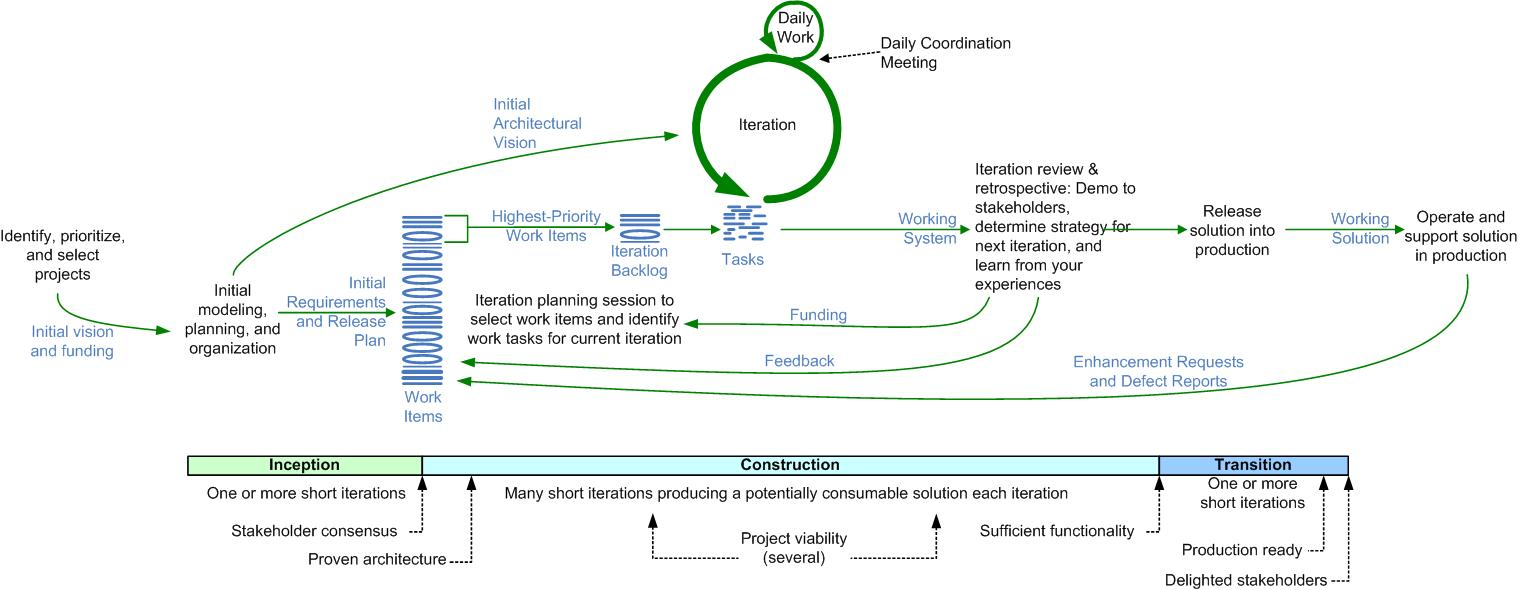
\includegraphics[width=1.0\textwidth]{dadLifecycleUP2}
  \caption{DAD basic Lifecycle}
\end{figure}
Mijlpalen :
\begin{enumerate}
\item Stakeholder consensus
\item Proven architecture
\item Sufficient functionality
\item Production ready
\item Delighted stakeholders
\end{enumerate}

\subsubsection{Iteratie aanpak}
\begin{itemize}
 \item Analyse : Modellen, requirements,  prioriteiten en selectie
 \item (Test Driven) Development
 \item Refactoring
 \item Peer review
 \item Levert steeds iets bruikbaars op dat ge\"evalueerd kan worden voor feedback.
 \item Planning
 \item Documentatie
\end{itemize}

%%
%% Dit is een subdocument van het projectplan.
%%
%% items op basis van SE Sommerville p623 (chapter 23.2.1 Project plans)
%%  	sommige items zijn elders in het document reeds opgenomen,  zoals bvb risico's
%%

\section{Planning}
\subsection{Indeling activiteiten over de drie DAD fasen}
%%zie Sommerville SE 2.4 The RUP (ed9 blz50-51)
\begin{enumerate}
\item \underline{\textbf{Inceptie (2 iteraties)}}
%%http://disciplinedagiledelivery.wordpress.com/2012/11/11/comparing-dad-to-the-rational-unified-process-rup-part-2/
		\begin{itemize}
		\item Iteratie ``Planning''
			\begin{itemize}
			\item Team afspraken.
			\item Stakeholder meeting.
			\item Probleem definitie.
			\item High level requirements.
			\item Planning.
			\end{itemize}
		\paragraph{Artefacten}
		De teamleden hebben de nodige afspraken gemaakt m.b.t. werkwijzen zoals
		communicatie middelen en versiebeheer voor documentatie. Deze fase levert
		een document dat het probleem omschrijft,  de high-level requirements,
		business case, risiso's, stakeholders, vision and challenges, een plan van
		aanpak en een planning voor de eerst volgende iteratie.
		\item Iteratie ``Domein onderzoek''
			\begin{itemize}
			\item Domein onderzoek.
			\item Requirements: Demonstratie van de huidige WickedXmas tool door
			stakeholder.
			\item Requirements: Op basis van sourcecode van de huidige WickedXmas tool.
			\item Initi\"ele architectuur visie
			\end{itemize}
		\paragraph{Artefacten}
		De resultaten van het domein onderzoek, eisen uit de observatie.
		De architectuur is bepaald en beschreven, het team heeft de IDE met tools
		ge\"{i}nstalleerd en getest.
		\end{itemize}


\item \underline{\textbf{Constructie (6 iteraties)}}
	\begin{itemize}
	\item Iteratie 0
		\begin{itemize}
		\item Modelling,  use cases
		\item Architectuur : afbakening,  onderdelen,  testen, evalueren
		\item documentatie aanpassen
		\end{itemize}
		\paragraph{Artefacten op de ``Proven architecture'' mijlpaal}
		 Architectuur getest en goed bevonden, documentatie
	\item Iteratie 1
		\begin{itemize}
		\item WickedXmas editor ontwikkelen
		\item documentatie aanpassen
		\end{itemize}
		\paragraph{Artefacten}
		Prototype, documentatie
	\item Iteratie 2
		\begin{itemize}
		\item WickedXmas editor ontwikkelen
		\item documentatie aanpassen
		\end{itemize}
		\paragraph{Artefacten}
		Prototype, documentatie
	\item Iteratie 3
		\begin{itemize}
		\item Start onderzoekcontext\footnote{De inhoud en diepgang van de onderzoekscontext is nog vaag. Dat moet na de 2e iteratie
		duidelijker zijn.}
		\item WickedXmas editor ontwikkelen
		\item documentatie aanpassen
		\end{itemize}
		\paragraph{Artefacten}
		Prototype, documentatie
	\item Iteratie 4
		\begin{itemize}
		\item WickedXmas analyse tool interface ontwikkelen
		\item documentatie aanpassen
		\end{itemize}
		\paragraph{Artefacten}
		Prototype, documentatie
	\item Iteratie 5
		\begin{itemize}
		\item WickedXmas analyse tool interface ontwikkelen
		\item documentatie aanpassen
		\end{itemize}
		\paragraph{Artefacten op de ``Sufficient functionality'' mijlpaal }
		 Een release van de WickedXmas Tool zoals beoogd werd,  documentatie
	\end{itemize}

\item \underline{\textbf{Finale transitie (1 iteratie)}}
	\begin{itemize}
		\item Finale releases van de nieuwe WickedXmas tool.
		\item Documentatie bundelen (handleiding).
		\item Onderzoekscontext afwerken.
		\item Presentatie geven
	\end{itemize}
	\paragraph{Artefacten op de ``Production ready'' mijlpaal}
	Een presentatie, documentatie, de nieuwe WickedXmas tool en de onderzoekscontext.

\end{enumerate}
%%
%% Dit is een subdocument van het projectplan.
%%
%%  hier worden tijden en eventueel personen toegekend aan activiteiten
%%


\subsection{Schedule}
 %% dit onderdeel moet vermoedelijk in het schedule plan

\pagebreak
\begin{landscape}
\newgeometry{top=0.5cm,left=0.5cm,bottom=0.5cm,right=-5cm}

\begin{figure}[hp]
\begin{ganttchart}[
   y unit chart=.9cm,
   today=4
 ]{0}{37}
 \gantttitle{2014}{15}
 \gantttitle{2015}{22} \\
 \gantttitlelist{38,...,52}{1}
 \gantttitlelist{1,...,22}{1} \\
 
 \ganttgroup{Inceptie}{1}{8} \\
 \ganttbar{Planning}{1}{4} \\
 
 \ganttmilestone{Planning}{4} \\
 
 \ganttbar{Domeinanalyse}{5}{8} \\
 
 
 \ganttmilestone{Domeinanalyse}{8} \\
 
 \ganttgroup{Constructie}{9}{28} \\
 
 \ganttbar{Iteratie 0}{9}{11} \\
 \ganttmilestone{Proven Architecture}{11} \\
 \ganttbar{Iteratie 1}{12}{14} \\
 \ganttbar{Iteratie 2}{17}{19} \\
 \ganttbar{Iteratie 3}{20}{22} \\
 \ganttbar{Iteratie 4}{23}{25} \\
 \ganttbar{Iteratie 5}{26}{28} \\
 
 \ganttmilestone{Constructie}{28} \\
 
 \ganttgroup{Transitie}{29}{31} \\
 \ganttbar{Onderzoekcontext}{20}{29} \\
 \ganttbar{Afronding}{30}{32}
 \ganttbar[bar/.style={fill=gray}]{}{32}{37} \\
 
 \ganttmilestone{Einde project}{37} 
 
 \ganttlink{elem1}{elem2}
 \ganttlink{elem2}{elem3}
 \ganttlink{elem3}{elem4}
 \ganttlink{elem4}{elem6}
 \ganttlink{elem6}{elem7}
 \ganttlink{elem7}{elem8}
 \ganttlink{elem8}{elem9}
 \ganttlink{elem9}{elem10}
 \ganttlink{elem10}{elem11}
 \ganttlink{elem11}{elem12}
 \ganttlink{elem12}{elem13}
 \ganttlink{elem9}{elem15}
 \ganttlink{elem13}{elem16}
 \ganttlink{elem15}{elem16}
 \ganttlink{elem17}{elem18}
 
\end{ganttchart}
\caption{Globale planning met hoofdfasen en belangrijkste mijlpalen}
\end{figure}

\pagebreak

\begin{figure}[hp]
\begin{ganttchart}[
    today=26
  ]{0}{32}
  \gantttitle{2014}{32} \\
  \gantttitle{september}{18}
  \gantttitle{oktober}{14} \\
  \gantttitlelist{13,...,30}{1}
  \gantttitlelist{1,...,14}{1}\\
  
  \ganttmilestone{Startbijeenkomst}{0.5} \\
  \ganttbar{Teamafspraken}{2}{7} \\
  \ganttbar{Stakeholder meeting}{8}{8} \\
  \ganttbar{Probleemdefinitie}{9}{24} \\
  \ganttbar{High-level requirements}{9}{24} \\
  \ganttmilestone{Concept planning}{27} \\
  
  \ganttbar{Verbeteringen}{28}{32} \\
  \ganttmilestone{Planning}{32}
  
  \ganttlink{elem0}{elem1}
  \ganttlink{elem1}{elem2}
  \ganttlink{elem2}{elem3}
  \ganttlink{elem2}{elem4}
  \ganttlink{elem3}{elem5}
  \ganttlink{elem4}{elem5}
  \ganttlink{elem5}{elem6}
  \ganttlink{elem6}{elem7}
 
\end{ganttchart}
\caption{Detailplanning 'Planning'}
\end{figure}

\pagebreak

\begin{figure}[hp]
\begin{ganttchart}[]{0}{33}
  \gantttitle{Domeinanalyse}{33}
  \ganttnewline
  \gantttitle{2014}{33} \\
  \gantttitle{oktober}{17}
  \gantttitle{november}{16} \\
  \gantttitlelist{14,...,31}{1}
  \gantttitlelist{1,...,14}{1}\\
  
  \ganttmilestone{Planning}{0.5} \\
  \ganttbar{Demonstratie WickedXmas}{2}{2} \\
  \ganttbar{Domeinanalyse GB}{3}{22}
  \ganttbar[bar/.style={fill=gray}]{}{23}{29} \\
  \ganttbar{Domeinanalyse JK}{3}{7}
  \ganttbar{}{13}{27}
  \ganttbar[bar/.style={fill=gray}]{}{28}{29} \\
  \ganttbar{Domeinanalyse SV}{3}{11}
  \ganttbar{}{19}{29} \\
  \ganttmilestone{Domeinanalyse}{30}
  
  \ganttlink{elem0}{elem1}
  \ganttlink{elem1}{elem2}
  \ganttlink{elem1}{elem4}
  \ganttlink{elem1}{elem7}
  \ganttlink{elem3}{elem9}
  \ganttlink{elem6}{elem9}
  \ganttlink{elem8}{elem9}
  
\end{ganttchart}
\end{figure}

%%\restoregeometry
\end{landscape}




\begin{tabular}{ll}\hline
{\bf Fase}    & {\bf weken}\\\hline
Planning             & 2,5 \\
\hline
Domeinanalyse        & 3 \\
Iteratie 0           & 3 \\
\hline
Iteratie 1           & 3 \\
Iteratie 2           & 3 \\
Iteratie 3           & 3 \\
Iteratie 4           & 3 \\
Iteratie 5           & 3 \\
\hline
Onderzoekcontext     &	2 \\
\hline
Afronding	     & 1.5 \\
\hline
Totaal               & 27 \\
\end{tabular}


\begin{itemize}
 \item 27 weken * 15 uur/week = 405 uur
 \item 8 maanden, ongeveer 32 weken beschikbaar, dus 5 weken marge
 \item Na elke iteratie wordt een voorlopige versie van de software aan de opdrachtgever verstrekt
\end{itemize}



\paragraph{Planning iteraties}

\begin{figure}[h]
 \begin{ganttchart}[
 ]{0}{21}
  \gantttitle{Planning iteraties}{21} \\
  \gantttitlelist{1,...,21}{1} \\
  \ganttbar{Requirements}{1}{7} \\
  \ganttbar{Ontwikkeling}{3}{18} \\
  \ganttbar{Documentatie}{10}{18} \\
  \ganttmilestone{Release}{18} \\
  \ganttbar{Scriptieverslag}{19}{20} \\
  \ganttbar{Evaluatie}{19}{20} \\
  \ganttbar{Onderzoekcontext}{19}{20} \\
  \ganttmilestone{Einde iteratie}{21}
 \end{ganttchart}
\end{figure}


Elke iteratie omvat een vaste periode van 3 weken.
In de eerste iteraties zal relatief meer tijd worden besteed aan requirements en
weinig tot geen aan de onderzoekcontext. In latere iteraties komt de onderzoekcontext
juist meer aan bod. Aan het einde van elke iteratie zijn twee dagen gereserveerd
voor het werken aan het scriptieverslag en de onderzoekcontext. In deze periode vindt
ook een evaluatie plaats van de afgelopen iteratie. \\
Voor het vaststellen van de requirements zal regelmatig overleg met Bernard plaats
moeten vinden. Hiervoor is het belangrijk dat in de detailplanning van een iteratie
rekening wordt gehouden met de beschikbaarheid van Bernard.


\todo[inline, color=blue!40, caption=planning]{Nu onderzoekcontext, documentatie en
scriptieverslag (deels) in de iteraties zijn opgenomen is er tijd vrijgekomen in de
planning. Hoe moeten we deze tijd invullen, iteraties langer of een extra iteratie?}




\begin{tabular}{lll}\hline
{\bf Week}    & {\bf Taak}  & {\bf Extra}\\\hline
38-41         & Planning    \\
42-45         & Domeinanalyse & 4 weken ingepland i.v.m. vakanties Stefan \& Jeroen \\
46-48         & Iteratie 0    \\
49-51         & Iteratie 1    \\
52-1          &               & geen iteratie i.v.m. vakantieperiode, mogelijk individueel (onderzoekcontext?) \\
2-4           & Iteratie 2    \\
5-7           & Iteratie 3    \\
8-10          & Iteratie 4    \\
11-13         & Iteratie 5    \\
14-16         &               \\
17-18         & Onderzoekcontext \\
19-20         & Afronding     \\
22            & Mijlpaal einde project

\end{tabular}




\paragraph{Capaciteitsplanning}

\begin{itemize}
 \item Beschikbare tijd
 \begin{itemize}
  \item $\sim$15 uur per week per teamlid
  \item $\sim$30 uur gedurende het hele project voor Freek en $\sim$20 uur voor Bernard
 \end{itemize}

 
 
 \item vakanties / niet beschikbaar voor project
 \begin{itemize}
  
  \item Stefan
  \begin{itemize}
   \item 25-10-2014 t/m 31-01-2014 (week 44)
   \item 24-12-2014 t/m 02-01-2015 (week 52-01)
  \end{itemize}
 
  \item Jeroen
  \begin{itemize}
   \item 21-10-2014 t/m 25-10-2014 (week 43)
  \end{itemize}
 
  \item Bernard
   \begin{itemize}
    \item 04-10-2014 t/m 14-10-2014 (week 41-42)
    \item 20-10-2014 t/m 27-10-2014 (week 43-44)
   \end{itemize}

 \end{itemize}
\end{itemize}


\subsection{Open punten}

\begin{enumerate}
 \item Is het de bedoeling dat de ontwerpen die met deze tool gemaakt kunnen worden ook voor de productie van een chip gebruikt zullen worden, m.a.w. bestaat er een risico dat fouten door deze tool leiden tot een fout geproduceerde chip?
 \item Wat is een onderzoekscontext?
 \item Aan welke eisen moet het scriptieverslag voldoen?
 \item Aan welke eisen moet de presentatie voldoen?
 \item Hoe gaan we agile precies invullen?
 \item Hoe valt Freek in de iteratie tijdens de uitvoering? Welke rol speelt Freek precies tijdens de andere fases?
 \item wat is het belang van i18n voor systeem documentatie?
 \item wat is het belang van l10n voor de software (variabele namen, menu opties)?
 \item moet de communicatie in meerdere talen aanwezig zijn?

 \item Open punten m.b.t. vision (zie sectie \ref{sec: vision} op pagina \pageref{sec: vision}).
 \begin{description}
  \item[Installatie] Moet het mogelijk zijn dat een draaiend tool zelf een update download en installeert (nice to have maybe)?
  \item[Dynamische controle] Moet het mogelijk zijn controles uit te schakelen of sequentieel te maken?
 \end{description}

 \item Open punten m.b.t. doelstellingen (zie sectie \ref{sec: challenges goals} op pagina \pageref{sec: challenges goals}).
 \begin{description}
    \item[ontwikkeltaal] Zijn er eisen aan de ontwikkeltaal of de ontwikkelomgeving?
    \item[ontwerp proces] Zijn er wensen ten aanzien van het ontwerp proces ten opzichte van het
	huidig gerealiseerde WickedXmas? Bijvoorbeeld parallelle verificatie en controle?
    \item[analyse tools] Zijn er wensen ten aanzien van de analyse tools zelf? Nieuwe analyse tool?
    \item[design functionaliteit] Zijn er nog meer wensen ten aanzien van design functionaliteit? Zoals parametrische queue sizes?
    \item[Multi user repository] Zijn er wensen ten aanzien van multi user repo?
 \end{description}
\end{enumerate}

\appendix
\section{Definitions}

\begin{description}
 \item[i18n] Internationalization, referring to translation of menu items, system documentation etc.
 \item[l10n] Localization, referring to country specific settings such as money, numbers, dates etc.
\end{description}
\section{Verwijzingen}

\bibliography{plan.bib}
\end{document} ;########################### end document ##################################;